\section{Applications and Experiments}
\label{sec:applications}

As outlined in Section~\ref{sec:introduction}, we report on three
applications of our framework.  From the least to the most sophisticated,
these are:
\begin{itemize}
\item sharing the cost of assertions among many users (Section~\ref{sec:ccured});

\item isolating a bug that is deterministic with respect to a predicate
(Section~\ref{sec:ccrypt});

\item using statistical regression techniques to isolate a bug that is non-deterministic with respect to every considered predicate (Section~\ref{sec:bc}).
\end{itemize}
For each application we report on the overhead of instrumentation.
For the last two applications we also quantify how effectively and efficiently
the bugs are isolated.  While the bug isolation examples presented here
are based on finding particular bugs in specific programs, 
the techniques are general.


\subsection{Sharing the Cost of Assertions}
\label{sec:ccured}

In conventional usage, C \texttt{assert()} calls are used during
program development but are disabled when code 
ships to boost performance.  However, deployed programs fail in
unanticipated ways, and it would be helpful to retain some level of
assertion checking if the performance penalty were not excessive.

The \CCured translator analyzes programs written in C and
attempts to prove that pointer operations are memory
safe.  Where this cannot be done, \CCured inserts dynamic checks to
enforce memory safety at run time \cite{POPL_'02*128}.  For our purposes, 
\CCured is simply a source of assertion-dense code.
The individual assertions are quite small and fast (array bounds
checks, testing for null, etc.)  but their performance impact can be
significant.  We wish to use random sampling to spread this cost
among many users.

We have applied sampling to \CCured versions of several Olden
\cite{Carlisle:1996:OPPWDDSDMM} and SPECINT95 \cite{SPEC95} benchmarks.
All programs run to completion and we are simply measuring
the overhead of performing the dynamic checks.

\subsubsection{Whole-Program Sampling}
\label{sec:share:whole}

\begin{table*}
  \centering
  \small
  \begin{tabular}{|l|rrr|rrr|}
    \hline
    & \multicolumn{3}{c|}{\textbf{function counts}} & \multicolumn{3}{c|}{\textbf{average for functions with sites}} \\
    \raisebox{1.5ex}[0pt]{\textbf{benchmark}} & \textbf{total} & \textbf{weightless} & \textbf{has sites} & \textbf{sites} & \textbf{threshold checks} & \textbf{threshold weight} \\
    \hline\hline
    \texttt{bh} & 64 & 15 & 48 & 11.9 & 3.8 & 9.5 \\
\texttt{bisort} & 13 & 3 & 10 & 4.1 & 1.9 & 2.6 \\
\texttt{em3d} & 15 & 5 & 10 & 5.5 & 3.1 & 4.7 \\
\texttt{health} & 16 & 2 & 14 & 6.1 & 2.9 & 3.1 \\
\texttt{mst} & 16 & 5 & 11 & 6.2 & 2.5 & 3.9 \\
\texttt{perimeter} & 11 & 4 & 6 & 7.8 & 2.7 & 2.1 \\
\texttt{power} & 19 & 4 & 15 & 5.8 & 3.0 & 2.8 \\
\texttt{treeadd} & 7 & 2 & 5 & 3.6 & 2.0 & 2.5 \\
\texttt{tsp} & 14 & 5 & 8 & 15.2 & 3.9 & 3.5 \\
\hline
\texttt{compress} & 20 & 4 & 15 & 7.1 & 2.9 & 3.9 \\
\texttt{go} & 380 & 12 & 359 & 14.8 & 6.0 & 4.7 \\
\texttt{ijpeg} & 314 & 34 & 267 & 18.7 & 5.0 & 7.3 \\
\texttt{li} & 375 & 16 & 336 & 6.2 & 3.2 & 2.9 \\
\hline

  \end{tabular}
  \caption{Static metrics for \CCured benchmarks.  Olden benchmarks
    are listed first, followed by SPECINT95.}
  \label{tab:share:static}
\end{table*}

Table~\ref{tab:share:static} summarizes static aspects of the sampling
transformation when applied to the entirety of each benchmark.  For
each program, we give the total number of non-library functions and
the number of these that are weightless.  As \CCured is a
whole-program analysis, weightless function identification has the
advantage of being able to examine every function body.  We also count
the number of functions that directly contain at least one
instrumentation site.  (The remainder are functions that have no sites
of their own but that call other non-weightless functions.)

Considering just the functions that directly contain at least one
instrumentation site, Table~\ref{tab:share:static} also presents the
average number of sites per function, the average number of threshold
check points per function, and the average threshold weight for all
such points.  (Note that the product of the last two of these metrics
may exceed the first, as a single instrumentation site may fall under
more than one threshold check point.  This can be seen in the example
in Figure~\ref{fig:code-layout} as well.)  The average site count
shows the density of assertions in the code.  The average
threshold weight measures how effective our transformation has been in
amortizing the cost of countdown checks over multiple sites.
Single-site functions are not uncommon; thus, an average threshold
weight above two is encouraging because it suggests that overall
amortization rates are good.

\begin{table}
  \centering
  \begin{tabular}{|l|r|rrrr|}
    \hline
    \rule{0pt}{2.5ex}
    \textbf{benchmark} & \textbf{always} & $\mathbf{10^{-2}}$ & $\mathbf{10^{-3}}$ & $\mathbf{10^{-4}}$ & $\mathbf{10^{-6}}$ \\
    \hline\hline
    \texttt{bh} & 2.81 & \textit{1.30} & \textit{1.10} & \textit{1.07} & \textit{1.07} \\
\texttt{bisort} & 1.08 & \textit{1.07} & \textit{1.05} & \textit{1.05} & \textit{1.04} \\
\texttt{em3d} & 2.14 & \textit{1.12} & \textit{1.04} & \textit{1.02} & \textit{1.04} \\
\texttt{health} & 1.02 & 1.03 & \textit{1.02} & \textit{1.02} & \textit{1.02} \\
\texttt{mst} & 1.25 & \textit{1.06} & \textit{1.04} & \textit{1.03} & \textit{1.04} \\
\texttt{perimeter} & 1.08 & 1.19 & 1.13 & 1.13 & 1.12 \\
\texttt{power} & 1.36 & \textit{1.07} & \textit{1.05} & \textit{1.04} & \textit{1.04} \\
\texttt{treeadd} & 1.13 & \textit{1.09} & \textit{1.09} & \textit{1.09} & \textit{1.11} \\
\texttt{tsp} & 1.05 & 1.17 & 1.16 & 1.15 & 1.14 \\
\hline
\texttt{compress} & 2.01 & \textit{1.21} & \textit{1.14} & \textit{1.14} & \textit{1.14} \\
\texttt{go} & 1.17 & 1.46 & 1.26 & 1.22 & 1.22 \\
\texttt{ijpeg} & 2.46 & \textit{1.17} & \textit{1.05} & \textit{1.04} & \textit{1.03} \\
\texttt{li} & 1.58 & \textit{1.24} & \textit{1.18} & \textit{1.16} & \textit{1.16} \\
\hline

  \end{tabular}
  \caption{Relative performance of \CCured benchmarks with
    unconditional or sampled instrumentation.  \textit{Italics} marks
    cases where sampled instrumentation outperforms unconditional
    instrumentation.}
  \label{tab:share:density}
\end{table}

Table~\ref{tab:share:density} shows the performance impact of
unconditional instrumentation as well as sampled instrumentation at
various densities.  The baseline for comparison is code
translated by \CCured and from which all dynamic memory
safety checks are removed.  We report the speedup ($>1$) or
slowdown ($<1$) relative to this baseline when sampling at various
densities.  All benchmarks were compiled using \texttt{gcc} 3.2 using
optimization level \texttt{-O2}.  Times were collected on a 1.3
GHz Pentium 4 Linux workstation with 512 megabytes of RAM\@.  Reported
speedups represent the average of four runs; each run used a different
pre-generated bank of 1024 geometrically distributed random
countdowns.

Unconditional instrumentation imposes slowdowns that vary widely from
(\texttt{health}: 2\%) to (\texttt{bh}: 181\%; \texttt{ijpeg}: 146\%).
Even at a fairly high sampling density of \nicefrac{1}{100}, more than
two thirds of our benchmarks run faster than when all checks are
always performed.  Because each single check is small and fast, this
suggests that we have been successful in amortizing the sampling
overhead.  On the other hand, three benchmarks run slower, with
\texttt{go} showing the largest penalty.  In these cases, the time
recovered by skipping \nicefrac{99}{100} checks is not enough to mask
the added overhead of sampling.  Furthermore, in all benchmarks, the
overhead relative to instrumentation-free code remains large.  Only
five benchmarks have less than a 10\% slowdown, and only one is below
5\%.

Performance improves as we reduce the sampling density to
\nicefrac{1}{1000}.  Most benchmarks suffer less than a 10\% penalty
relative to uninstrumented code, and half are below 5\%.  Further
reducing the sampling density to \nicefrac{1}{10,000} shows little
change, and by the time we reach \nicefrac{1}{1,000,000} it is clear
that we have reached a performance floor.  Three benchmarks
(\texttt{perimeter}, \texttt{tsp}, \texttt{go}) are unable to
compensate for their sampling overhead relative to unconditional
instrumentation, while the remaining ten do run faster.  Among these,
a few benchmarks (\texttt{treeadd}, \texttt{compress}, \texttt{li})
retain high overhead relative to instrumentation-free code, but in
most cases the penalty is quite modest.  Some benchmarks that perform
the worst using unconditional instrumentation perform quite well with
sampling: \texttt{ijpeg}, for example, moves from an unconditional
instrumentation overhead of 146\% to only 3\% with sparse sampling.

\subsubsection{Statically Selective Sampling}
\label{sec:ccured:single}

It is not necessary to put
all instrumentation into a single executable; one can easily 
create multiple executables where each contains a subset of the complete
instrumentation.  Partitioning instrumentation by site, by module, by
function, or by object file are all reasonable schemes.  Any
individual executable contains less instrumentation and therefore
incurs a smaller performance penalty.  Fewer sites mean more
weightless functions, and therefore better interprocedural
optimization per Section~\ref{sec:framework:calls}.  Functions without
instrumentation sites require no code duplication, which limits
executable growth.  Known trusted code can be exempted from
instrumentation, or especially suspect code can be ``farmed out'' to a
larger proportion of users for more intensive study.  Given a suitable
dynamic instrumentation infrastructure, sites can be added or removed
over time as debugging needs and intermediate results warrant.

\begin{sloppypar}
  We have experimented with variants of the \CCured benchmarks in
  which only a single function is instrumented at a time.  Whereas
  fully instrumented executables range from 13\%-149\% larger than
  their non-sampling counterparts, average growth for single-function
  instrumented executables is just 12\% for the small Olden benchmarks
  and 6\% for the larger SPECINT95 applications.  Performance is uniformly good:
 at \nicefrac{1}{1000} sampling,  94\% of site-containing functions incur less than 5\% slowdown
  versus instrumentation-free code, while even the worst single
  function has less than a 12\% penalty.
\end{sloppypar}

\subsubsection{The Effectiveness of Sampling}

From these benchmarks and the examples in Sections~\ref{sec:ccrypt}
and~\ref{sec:bc}, we conclude that realistic deployments will use
sampling densities between \nicefrac{1}{100} and \nicefrac{1}{1000}.
But how effective is \nicefrac{1}{1000} sampling at observing rare
program behavior?  Suppose we are interested in a bug occurring once
per hundred executions.  To achieve 90\% confidence of observing this
bug in at least one run, we need at least
%%
\[\log{(1-0.90)} / \log{\left( 1 - \frac{1}{100 \times 1000}\right)} = \text{230,258 runs.}\]

While this is a large number, consider that sixty million Office XP
licenses were sold in its first year on the market
\cite{Microsoft:2002:AR-F10K}.  Assuming each licensee runs Microsoft
Word twice per week, then this user base produces 230,258 runs every
nineteen minutes.  Achieving 99\% confidence of observing a 
bug that occurs on one in a thousand runs requires 4,605,168 runs, 
which takes less than seven hours to gather.  

For smaller deployments, we must either wait longer for sufficient
data or increase the sampling density.  As we shall see in
Sections~\ref{sec:ccrypt} and~\ref{sec:bc}, at least for restricted
classes of bugs we can perform useful analysis with a few thousand
executions.  Thus, our techniques are likely most suited to
applications where it is possible to gather data with at least  \nicefrac{1}{1000} sampling from thousands of executions per day.


\subsection{Bug Isolation Using Predicate Elimination}
\label{sec:ccrypt}

In this section we consider automatic isolation of deterministic
bugs.  Recall from Section~\ref{sec:introduction} that for a deterministic
bug there is a predicate that becomes true
if the program must crash at some point in the future.
Deterministic bugs are quite common, though they are generally easier
to find and fix using any method than non-deterministic bugs (see
Section~\ref{sec:bc}).

\subsubsection{Instrumentation Strategy}

As a case study in finding deterministic bugs we take release 1.2 of
the \texttt{ccrypt} encryption tool.  This version is known to contain
a bug that involves overwriting existing files.  If the user responds to
a confirmation prompt with
\texttt{EOF} rather than \texttt{yes} or \texttt{no}, \texttt{ccrypt}
crashes.

The \texttt{EOF} sensitivity suggests that the problem has something to do with
\texttt{ccrypt}'s interactions with standard file operations.
In C, these functions commonly return values to indicate
success or failure.  Many C application programmers follow the same
model for their own error reporting.  Thus, randomly sampling function
return values may identify key operations that behave differently in
successful versus crashed runs.  We group function return values into
three classes: negative values, zero, and positive values.  This
reduces the amount of information we must track while still making
distinctions consistent with common C programming style.

We instrument \texttt{ccrypt} as follows.
Consider each syntactic call site that returns
scalar values, including both arithmetic types as well as pointers.
After each such call, update one of three counters depending upon the
sign of the result: one for negative values, one for zeros, and one
for positive values.  Each call site has its own triple of counters.
Thus, when the program terminates, we can examine any function call of
interest and ask how often that call returned a negative, zero, or
positive value.  

For \texttt{ccrypt}, there are 570 call sites of interest, for $570 \times 3 =
1710$ counters.  Each counter corresponds to a single predicate that
is hypothesized to behave differently in successful versus crashed
runs.  Specifically, we pose the problem as follows:
\begin{quote}
  Assume that predicates capture incorrect behavior.  That is, assume
  that each predicate $P$ should always be false during correct
  execution.  When $P$ is true, the program either fails (a deterministic
bug) or is at
  increased risk of failing (a non-deterministic bug).
\end{quote}

If we eliminate all predicates for which this hypothesis is disproved
by observed runtime behavior, then the predicates that remain
describe the conditions under which the program fails.

\subsubsection{Elimination Strategies}

We make no effort to restrict instrumentation to known
system or library calls, nor do we distinguish
functions that return status codes from those that do not.  
Most of those 1710 predicates,
then, have no bearing on program success or failure.
Given a set of runs, we can discard irrelevant predicates using a 
set of \termdef{elimination strategies}:

\begin{elimlist}
  \begin{sloppypar}
  \item[\elim{Elimination by universal falsehood}:] Disregard any
    counter that is zero on all runs.  These likely represent
    predicates that can never be true.
  \end{sloppypar}

\item[\elim{Elimination by lack of failing coverage}:] Disregard any
  triple of counters all three of which are zero on all failed runs.
  Because one counter in each triple must always be true for any
  sample, these likely represent instrumentation sites that are not
  even reached in failing executions.
  
\item[\elim{Elimination by lack of failing example}:] Disregard any
  counter that is zero on all failed runs.  These likely represent
  predicates that need not be true for a failure to occur.
  
\item[\elim{Elimination by successful counterexample}:] Disregard any
  counter that has a non-zero value on any successful run.  These
  must represent predicates that can be true without a subsequent
  program failure.
\end{elimlist}

We characterize these as strategies because they are subject to noise
from random sampling, and also because not all are equally applicable
to all bugs.  For example, elimination by \elim{successful
  counterexample} assumes that the bug is deterministic.  The other three
strategies do not make this assumption, but do require enough
runs so that any predicate that is ever true is likely to
have been observed true at least once.  Note that these
strategies are also not independent: \elim{universal falsehood} and
\elim{lack of failing coverage} each eliminate a subset of the
counters identified by \elim{lack of failing example}.  Elimination
strategies also vary in which kinds of runs they exploit:
\elim{successful counterexample} considers only successful runs;
\elim{lack of failing example} and \elim{lack of failing coverage}
consider only failures; \elim{universal falsehood} uses both.

\subsubsection{Data Collection and Analysis}

One function call, with one update to one of three counters, is considered one
instrumentation site.  We transform the instrumentation to be sampled
rather than unconditional using the framework described in
Section~\ref{sec:framework}.  In lieu of a large user community, we
generate many runs artificially in the spirit of the Fuzz
project~\cite{MKLMMNS95}.  Each run uses a randomly selected set of
present or absent files, randomized command line flags, and randomized
responses to \texttt{ccrypt} prompts including the occasional
\texttt{EOF}.

We have collected 2990 trial runs at a sampling rate of
\nicefrac{1}{1000}; 88 of these end in a crash.  Applying each
elimination strategy independently to the counter traces:

\begin{elimlist}
\item[\elim{Universal falsehood}] discards 1569 counters that are
  zero on all runs, leaving 141 candidate predicates.
  
\item[\elim{Lack of failing coverage}] discards 526 counter triples
  that are all zero on all crashes, leaving 132 candidate predicates.
  
\item[\elim{Lack of failing example}] discards 1665 counters that are
  zero on all crashes, leaving 45 candidate predicates.
  
\item[\elim{Successful counterexample}] discards 139 counters that
  are non-zero on any successful run, leaving 1571 candidate
  predicates.
\end{elimlist}

\begin{sloppypar}
  %% Several factors conspire to drive most counters to zero: the \naive
  %% nature of our guesses, the limited coverage of our automated test
  %% suite, and the filtering effect of sparse sampling.  Thus, 
  At first glance, elimination by \elim{universal falsehood} is quite
  effective while elimination by \elim{successful counterexample}
  seems rather poor.  However, these two strategies test disjoint
  properties and can be combined to good effect.  The combination
  leaves only those predicates that are sometimes observed to be true
  in failed runs but never observed to be true in successful runs.
  For our \texttt{ccrypt} trials, only two predicates meet this
  criterion:
\end{sloppypar}

\begin{features}
\item traverse.c:320: file\_exists() return value > 0
\item traverse.c:122: xreadline() return value == 0
\end{features}

Examining the corresponding code shows that these predicates are
consistent with the circumstances under which the bug is reported to
occur.  This call to \texttt{file\_exists()} returns ``\texttt{1}'' when an output
file already exists.  A confirmation prompt is presented, and this
call to \texttt{xreadline()} returns the user's reply, or null if the
input terminal is at \texttt{EOF}.  Inspection of the code immediately
following the \texttt{xreadline()} call shows that the programmer
forgot to check for the \texttt{EOF} case: he assumes that
\texttt{xreadline()} returns a non-null string, and immediately
inspects its contents.  We have successfully isolated this (known) bug
in \texttt{ccrypt}, and the fix is clear.

While the \texttt{file\_exists()} predicate is not itself the cause of
the bug, the fact that it appears on our list is useful information.
It represents a necessary condition under which crashes occur.  That
may be helpful, for example, if the engineer wishes to reproduce the
bug in-house for further study.  Of course, there should be some runs
where \texttt{file\_exists()} reports that the file exists but
\texttt{xreadline()} returns a valid response from the user and
therefore the program does not crash.  If the \texttt{file\_exists()}
call is sampled on such a run, elimination by \elim{successful
  counterexample} correctly concludes that this predicate does not
imply failure.  It will be eliminated from further consideration, and
only the true ``smoking gun,'' the call to \texttt{xreadline()}, will
remain.  Thus we have the ability to identify not only the direct
cause of a bug but also related behaviors that are strongly but
imperfectly correlated with failure.  We further explore this idea of
broad correlation in Section~\ref{sec:bc}, where even the buggy line
of code itself does not always cause a crash.

As previously noted, the first three elimination strategies partially
overlap, whereas the last, \elim{successful counterexample}, is
distinct.  \elim{Universal falsehood} and \elim{successful
  counterexample} only look at successful runs, hence are easily
analyzed together.  \elim{Lack of failing example} in general
eliminates the most features, and therefore is also a good candidate
to combine with \elim{successful counterexample}.  Doing so in the
case of \texttt{ccrypt} leaves us with exactly the same two features,
though in general one might find different results.  Elimination by
\elim{lack of failing coverage}, on the other hand, is an inherently
weaker strategy: when combined with \elim{successful counterexample},
we are still left with 86 features.

\subsubsection{Refinement over time}

In order to gain a better understanding of how the elimination
strategies benefit from increasing the number of runs, we have
experimented with randomized subsets of our complete run suite.  We
have seen that elimination by \elim{successful counterexample} is
quite effective when given a few thousand successful runs; how well
does it perform with a smaller suite?  We start with the 141 candidate
predicates that are ever nonzero on any run.  We assemble a random
subset of fifty successful runs and filter the predicate set using
elimination by \elim{successful counterexample}.  We then add another
fifty runs, and another fifty, and so on in steps up to the full set
of 2902 successful runs.  We repeat this entire process one hundred
times to gauge how rapidly one can expect the predicate set to shrink
as more runs arrive over time.

\begin{figure}
  \centering
  \small
  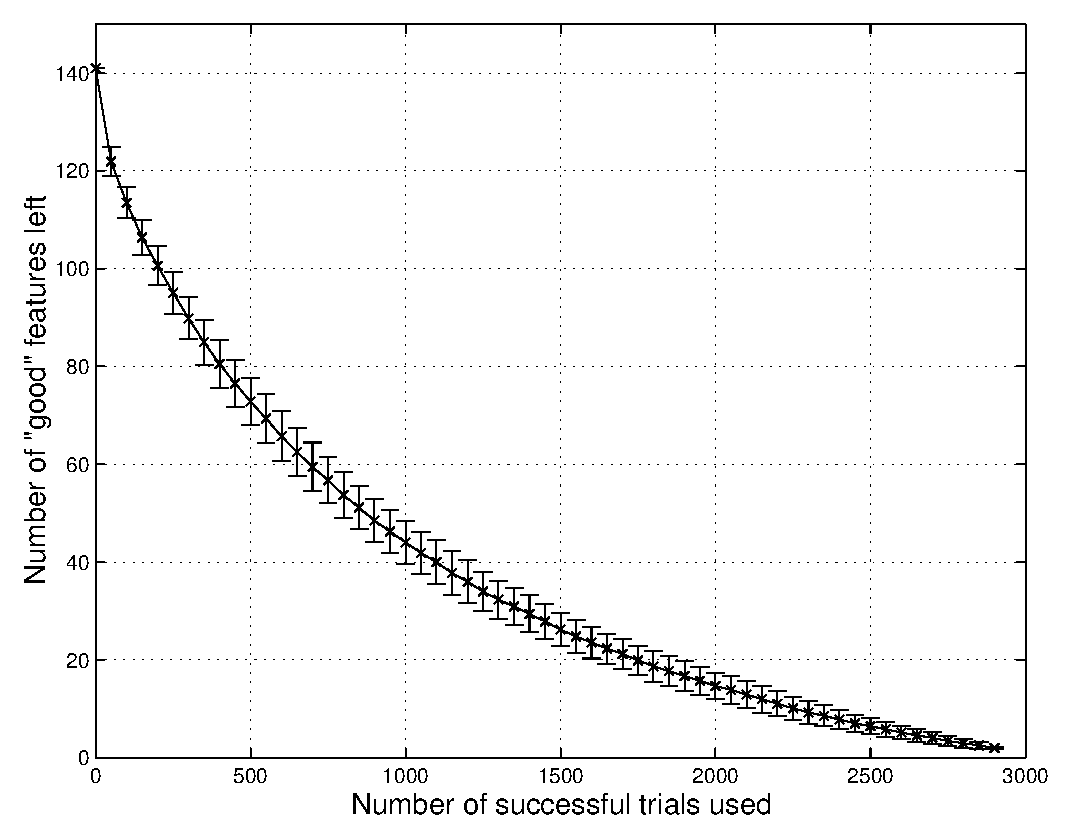
\includegraphics[width=\columnwidth]{applications/ds1000ngood_plot}
  \caption{Progressive elimination by \elim{successful counterexample}
    as successful runs accumulate.  Crosses mark means; error bars
    mark one standard deviation.}
  \label{fig:ngood}
\end{figure}

Figure~\ref{fig:ngood} shows the results.  The crosses mark the mean
number of predicates remaining, while the vertical bars extend one
standard deviation above and below the mean.  The short vertical bars
in this case tells us that there is relatively little diversity in
each of the hundred random subsets at any given size.  The results
show that, on average, 1750 runs are enough to isolate twenty
candidate features, another 500 runs reduces that count by half, and a
total of 2600 runs is enough to narrow the set of good features down
to just five.  One would expect more variety in runs collected from
real users rather than an automated script.  Greater diversity can
only benefit the analysis, as it would provide more novel
counterexamples and therefore may eliminate more uninteresting
predicates more rapidly.

\subsubsection{Performance Impact}

Instrumenting function return values confounds several of the
optimizations proposed in Section~\ref{sec:framework}.  If most
function calls are instrumentation sites, and if most function calls
terminate acyclic regions, then most acyclic regions contain only a
single site and we have poor amortization of sampling overhead.
Furthermore, \texttt{ccrypt} is built one object file at a time, and
we must conservatively assume that any cross-object function call is
not weightless.  Thus, for much of \texttt{ccrypt}, our sampling
transformation devolves to a simpler but slower pattern of checking
the next-sample countdown at each and every site.

%\begin{figure}
%  \centering
%  \small
%  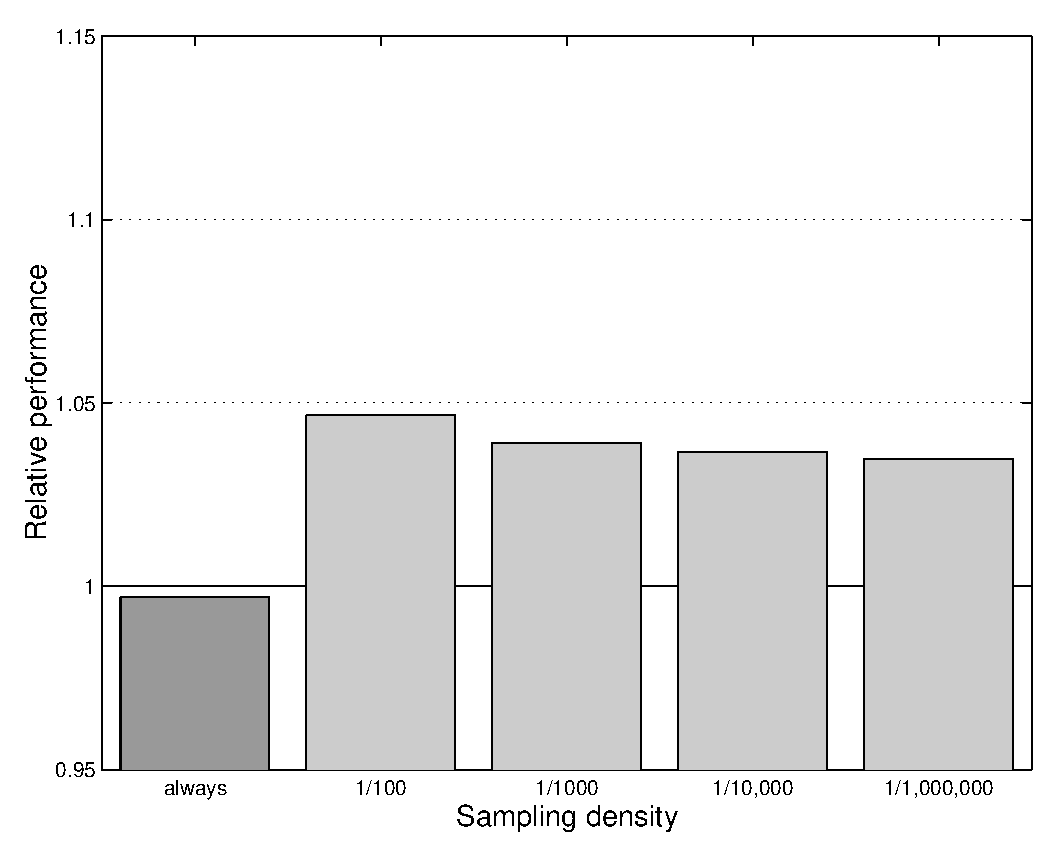
\includegraphics[width=\columnwidth]{applications/ccrypt_density}
%  \caption{Relative performance of \texttt{ccrypt} with unconditional or
%    sampled instrumentation}
%  \label{fig:ccrypt:slowdown}
%\end{figure}

In spite of this, the performance impact of sampled instrumentation is
minimal.  Using an experimental setup similar to that described
earlier in Section~\ref{sec:share:whole}, we find that the overhead
for \nicefrac{1}{1000} sampling is less than 4\%, and progressively
sparser sampling rates shrink this still further.  Unconditional
instrumentation also performs well here, making either reasonable for
this particular application.  In the next section, though, we consider
a more invasive instrumentation strategy that requires sampling to
keep overhead under control.

\subsection{Statistical Debugging}
\label{sec:bc}

In this section we consider the automatic isolation of non-deterministic
bugs.  Recall from Section~\ref{sec:introduction} that a bug is
non-deterministic with respect to a set of program predicates if no predicate
in the set is perfectly correlated with program crashes.  
For this case study we use version 1.06 of the GNU implementation of
\texttt{bc}.  We find that feeding \texttt{bc} nine megabytes of
random input causes it to crash roughly one time in four from, as it
turns out, a previously unknown buffer overrun error.  Since \texttt{bc}
sometimes terminates successfully even when it overruns the buffer,
this bug is non-deterministic.

We instrument \texttt{bc} using a variation on our previous strategy
of counter triples.  We abandon elimination by \elim{successful
counterexample}\footnote{Because the bug is non-deterministic, if we
have enough runs no predicates will satisfy elimination by
\elim{successful counterexample}.} in favor of statistical modeling to
identify behavior that is broadly correlated with failure.

\subsubsection{Instrumentation Strategy}

We instrument \texttt{bc} to guess and randomly check a large number
of predicates.  As before, our goal is to identify predicates
that capture bad behavior: false when the program succeeds and true
when the program crashes.  We cast an extremely broad net, but with an
eye toward pointer and buffer errors.  For pointers,
null pointers are of interest.  Relative addresses of pointers
may be interesting as well, as this may capture cases where one
pointer scans within a second pointed-to buffer.  Checking
pointer/pointer equality may reveal aliasing that, when not
anticipated by the programmer, can lead to dangling ``wild'' pointer
bugs.  Scalar variables serve as array indexes, pointer offsets, and
in many other roles; relationships among scalars may reveal buffer
overruns, unanticipated consequences of negative values, invalid
enumeration constants, or a variety of other problems.

At any direct assignment to a scalar variable \texttt{a}, we identify
all other local or global variables $\{ \mathtt{b}_1, \mathtt{b}_2,
\dots, \mathtt{b}_n \}$ that are also in scope and that have the
same type.  We then compare the updated \texttt{a} to each
$\mathtt{b}_i$, and note whether \texttt{a} was less than, equal to,
or greater than $\mathtt{b}_i$.  We compare pointers to same-typed
pointers as well, and additionally compare each pointer for equality
with null.  One comparison between \texttt{a} and $\mathtt{b}_i$,
which bumps one of three counters, is considered to be one
instrumentation site subject to random sampling.  When an instrumented
application terminates, it emits the vector of counter triples along
with a flag indicating whether it completed successfully or was
aborted by a fatal signal.

For \texttt{bc} there are 10,050 counter triples, or 30,150 counters
in all.  The vast majority of these are of no interest: either they
compare completely unrelated variables, or they express relationships
that behave identically in both successful and failed runs.  The
challenge is to find the few predicates that matter.

\subsubsection{Crash Prediction Using Logistic Regression}

To find the important predicates, we recast bug isolation as a
statistical analysis problem.  Each run of \texttt{bc} constitutes one
sample point consisting of 30,150 observed \termdef{features}
(counters) and one binary \termdef{outcome} ($0 = \text{succeeded}, 1
= \text{crashed}$).  Given numerous data points (sampled runs), we
want to identify a subset of our 30,150 features that predict the
outcome.  This is equivalent to the machine learning problem of
learning a binary classifier with feature selection, i.e., using as
few input features as possible.

In the classification setting, we take a set of data with known binary
output (a training set), and attempt to learn a binary classifier that
gives good predictions on a test set.  The learning process usually
involves additional parameters whose values can be determined using a
cross-validation set.  In our case, the end goal is to narrow down the set
of features.  Hence our method must balance good
classification performance with aggressive feature selection.

A binary classifier takes feature values as inputs, and outputs a
prediction of either $0$ or $1$.  \termdef{Logistic regression}
\cite{Hastie01} is a method of learning a binary classifier where the
output function is assumed to be logistic.  The logistic function is a
continuous ``S''-shaped curve approaching 0 on one end, and 1 on the
other.  The output can be interpreted as a probability measure of how
likely it is that the data point falls within class 0 or 1.  Quantizing the
logistic function output then gives us a binary classifier: if the
output is greater than \nicefrac{1}{2}, then the data point is
classified as class 1 (a crash), otherwise it falls under class 0 (a
successful run).  Feature selection can be achieved by
\termdef{regularizing} the function parameters to ignore most input
features, forcing it to form a model that predicts success or failure
using just a small selection of sampled features.  Regularization is
important for our purposes because we expect that most of our features
are wild guesses, but that there may be just a few that correctly
characterize the bug.

While other techniques for combined classification and feature
selection exist, few of them are particularly well-suited for this
problem.  Some methods \cite{Golub:MCC:1999,Tibshirani2002} calculate
a univariate correlation coefficient independently for each feature;
other methods, such as decision trees \cite{00000048}, are more
computationally intensive.  In our dataset, the features are clearly
not independent of each other, and the size of the problem can
potentially be too large for more computationally intensive methods.
Furthermore, logistic regression is a discriminative classification
method, and thus does not make any assumptions about the underlying
distribution of the input.  This is crucial since our features arise
from a decidedly artificial process and would be difficult to
characterize using simple distributions.

Suppose our training set $\mathcal{D}$ consists of $M$ data points
$(x_1,y_1), \ldots, (x_M, y_M) $, where each $x_i \in \Real^N$ denotes
a vector of input predicate counters, and each $y_i = \{0, 1\}$
denotes the corresponding output label.  To learn a good classifier,
we can maximize the \termdef{log likelihood} of the training set.
%%
\begin{equation*}
  \begin{split}
    LL(\mathcal{D}) \:=\:
    \sum_{i=1}^M \, [ & y_i \log P(Y = 1 | x) \\
    + & (1 - y_i) \log (1 - P(Y = 1 | x)) ].
  \end{split}
\end{equation*}

Here the output labels $y_i$ are used as indicator functions to zero
out exactly one of the two terms in each summand.  In logistic
regression, the distribution $P(Y=1|x)$ is modeled as the logistic
function $\mu_{\tilde{\beta}}(x)$ with parameters $\tilde{\beta} = \langle \beta_0 \in
\Real, \beta \in \Real^N \rangle$.
%%
\begin{equation*}
  P(Y = 1 | x) = \mu_{\tilde{\beta}} (x) = \frac{1}{1 + \exp(- \beta_0 - \beta^T x)}.
\end{equation*}

The logistic parameters $\beta_0$ and $\beta$ take on the respective roles as
the intercept and slope of the classifier, and essentially weigh the
relative importance of each feature in the final outcome.  We expect
most of the input features to have no influence over the success or
failure of the program, so we place an additional constraint that
forces most of the $\beta$'s toward zero.  This is accomplished by
subtracting a penalty term based on the $\ell_1$ norm $\norm{\tilde{\beta}}_1 =
\sum_{j=0}^M \abs{\beta_j}$.  We can tune the importance of this
\termdef{regularization term} through a \termdef{regularization
  parameter} $\lambda$.  The penalized log likelihood function is:
%%
\begin{equation*}
  \begin{split}
    LL (\tilde{\beta} | \mathcal{D}, \lambda ) \:=\:
    & \sum_{i=1}^M \, [y_i \log \mu_{\tilde{\beta}} (x_i) + (1 - y_i) \log (1 - \mu_{\tilde{\beta}} (x_i))] \\
    & - \lambda \norm{\tilde{\beta}}_1.
  \end{split}
\end{equation*}

An assignment of $\beta$ coefficients that maximizes this function
represents a model that maximizes the fidelity of its predictions
while still limiting itself to form those predictions on the basis of
only a small number of features from the complete feature set.

\subsubsection{Data Collection and Analysis}

Our \texttt{bc} data set consists of 4390 runs with distinct random
inputs and distinct randomized \nicefrac{1}{1000} sampling.  
We randomly chose 2729 runs for training, 322 runs for cross-validation, and 1339 runs
for testing.  Although there are 30,150 raw features, many can be
discarded immediately using elimination by \elim{universal falsehood}:
in the training set 27,242 features are always zero.  Hence the
effective number of features used in training is 2908.  (Elimination
by \elim{lack of failing example} can eliminate another 647 features
that are zero for all failed runs.  However we find that the presence
or absence of these 647 features does not significantly affect the
quality of the regularized logistic regression results.)

To make the magnitude of the $\beta$ parameters comparable, the feature
values must be on the same scale.  Hence all the input features are
shifted and scaled to lie on the interval $[0, 1]$, then normalized to
have unit sample variance.  A suitable value for the regularization
parameter $\lambda$ is determined through cross-validation to be $0.3$.  The model
is then trained using stochastic gradient ascent to reach a local
maximum of the penalized log likelihood.  Using a step size of
$10^{-5}$, the model usually converges within sixty iterations through
the training set.  This takes roughly thirty minutes in MATLAB on a
1.8 GHz Pentium 4 CPU with 1 GB of RAM.

Once the model has been trained, predicates with the largest $\beta$
coefficients suggest where to begin looking for the bug.  In our case,
the top five ranked coefficients are well-separated in magnitude from
the rest, and show an unmistakable trend:

\begin{features}
\item storage.c:176: more\_arrays(): indx > scale
\item storage.c:176: more\_arrays(): indx > use\_math
\item storage.c:176: more\_arrays(): indx > opterr
\item storage.c:176: more\_arrays(): indx > next\_func
\item storage.c:176: more\_arrays(): indx > i\_base
\end{features}

\begin{figure}
  \centering
  \VerbatimInput[frame=single,numbers=left,firstnumber=152,fontsize=\scriptsize,xleftmargin=24pt,xrightmargin=12pt]{applications/more_arrays.c}
  \caption{Suspect \texttt{bc} function \texttt{more\_arrays()}.  All
  top-ranked crash-predicting features point to large values of
  \texttt{indx} on line 176.}
  \label{fig:bc:more-arrays}
\end{figure}

The source code for \texttt{more\_arrays()} appears in
Figure~\ref{fig:bc:more-arrays}.  A comment earlier in the same file
suggests that this one of a suite of ``three functions for increasing
the number of functions, variables, or arrays that are needed.''  The
logic is a fairly clear instance of the buffer reallocation idiom,
even to one unfamiliar with the code: line 167 allocates a larger
chunk of memory; line 171 is the top of a loop that copies values over
from the old, smaller array; line 176 completes the resize by zeroing
out the new extra space.  As the comment suggests, there are two
similar functions (\texttt{more\_functions()} and
\texttt{more\_variables()}) nearby that do largely the same thing with
different storage pools.  The text of these three functions is nearly
identical, but each uses different global variables (such as
\texttt{a\_count} versus \texttt{f\_count} versus \texttt{v\_count}).

The top ranked predicates seem bizarre at first glance, because the
variables they relate do not appear to have any real connection to
each other or to \texttt{more\_arrays()}.  For example, \texttt{scale}
tracks significant digits for floating point calculations, while
\texttt{use\_math} records whether an initial math library is to be
loaded.  Why would crashes tend to happen when local variable
\texttt{indx} exceeds these seemingly unrelated globals on this
particular line?  An obvious hypothesis is that \texttt{indx} is
simply unusually large in such cases.  If \texttt{indx} is large, then
it will tend to be larger than any number of otherwise unrelated
variables.  Perhaps crashes occur when the input to \texttt{bc}
defines unusually large numbers of arrays.

Closer scrutiny of \texttt{more\_arrays()} quickly reveals this to be
the case.  The allocation on line 167 requests space for
\texttt{a\_count} items.  The copying loop on line 171 ranges from
\texttt{1} through \texttt{old\_count - 1}.  The zeroing loop on line
176 continues on from \texttt{old\_count} through \texttt{v\_count -
  1}.  And here we find the bug: the new storage buffer has room for
\texttt{a\_count} elements, but the second loop is incorrectly bound
by \texttt{v\_count} instead.  After a glimpse at the
neighboring \texttt{more\_variables()} function it is clear that
\texttt{more\_arrays()} was created by copying and pasting
\texttt{more\_variables()} and then changing names like
\texttt{v\_count} and \texttt{v\_names} to \texttt{a\_count} and
\texttt{a\_names}.  The loop bound on line 176 was missed in the
renaming.

The logistic regression model points us at the buggy line, the buggy
variable, and even reveals something of the conditions under which the
bug appears.  Having found the bug, it is reasonable to ask
whether the statistical analysis could have pointed at it even more
directly.  The mistaken use of \texttt{v\_count} instead of
\texttt{a\_count} on line 176 means that a buffer overrun occurs when
\texttt{indx > a\_count} on line 176.  This does correspond to a
predicate sampled by our system, but this predicate is ranked 240th in
the trained model.  Why was this, the smoking gun, not ranked first?

There are several reasons to consider.  Samples are taken randomly,
while the model itself is trained using stochastic gradient ascent.
Thus, a degree of noise is fundamental to the process.  Even crashing
is not guaranteed: out of 320 runs in which sampling spotted
\texttt{indx > a\_count} at least once, 66 did not crash.  Thus, C
programs can ``get lucky'', meaning that this is not a strict
$\text{overrun} \implies \text{crash}$ implication.  Manual inspection
of the data reveals a high degree of redundancy among many
instrumentation sites within \texttt{more\_arrays()}, meaning that the
model has several features to choose from that have equivalent
predictive power.  This suggests that our counters may be too
fine-grained---we are distinguishing many behaviors that are in
fact so tightly interrelated as to be equivalent.  
%Improving our
%instrumentation scheme and fine-tuning the statistical analysis
%methodology are key areas for continued development.

This bug seems clear enough once found.  However it has been present
and undiscovered at least since 1992 (the time\-stamp on this file in
the oldest version of GNU \texttt{bc} that we can find).  Many bugs
are obvious only once one knows where to look.  The logistic
regression results directed us to one misbehaving variable on one line
of code, out of 8910 lines in \texttt{bc} as a whole.  Our approach
does not automatically find and fix bugs.  But it does suggest where
to start looking, and what sort of scenarios (e.g., unusually large
\texttt{indx}) to consider.  Although we are still learning about the
capabilities of this system, and how to interpret its results, we
believe that statistically guided debugging has the potential to make
the process of finding and fixing bugs more efficient.

\subsubsection{Performance Impact}

\begin{figure}
  \centering
  \small
  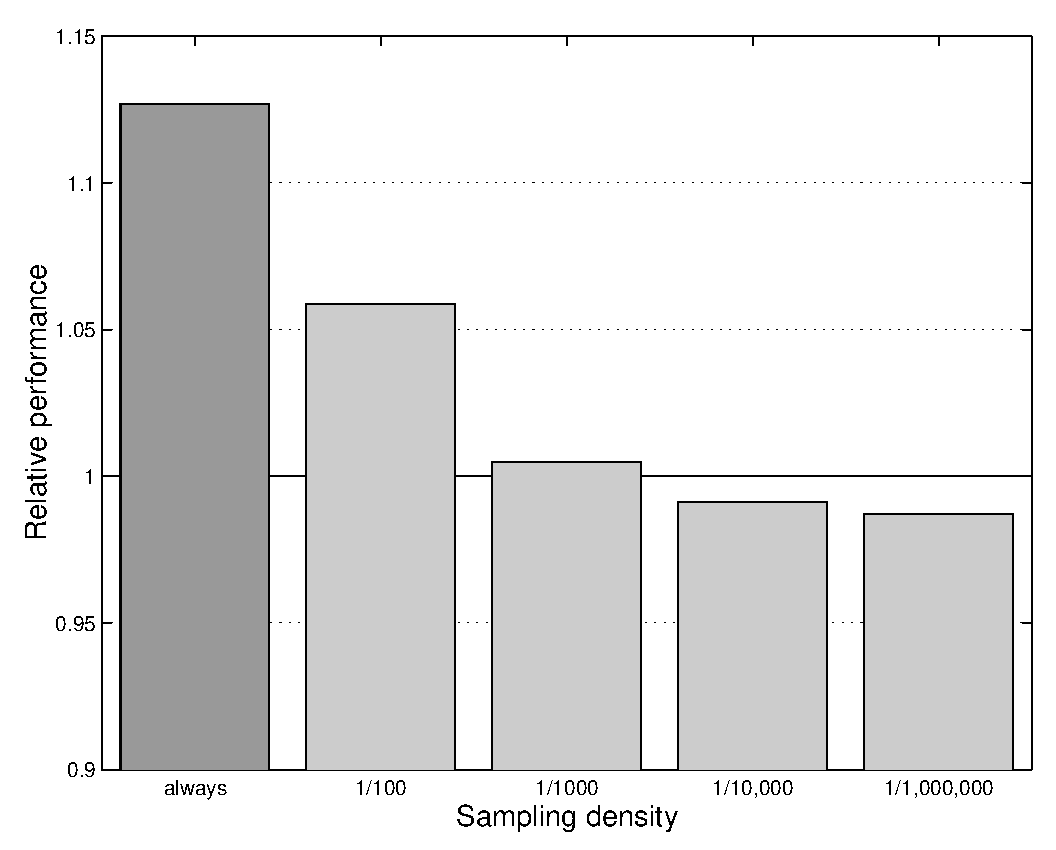
\includegraphics[width=\columnwidth]{applications/bc_density}
  \caption{Relative performance of \texttt{bc} with unconditional or
    sampled instrumentation}
  \label{fig:bc:slowdown}
\end{figure}

Our \texttt{bc} instrumentation is fairly dense.  The leftmost bar in
Figure~\ref{fig:bc:slowdown} shows that if this instrumentation is
added without sampling, the performance penalty is 
13\%.  A sampling density of \nicefrac{1}{100} cuts this in
half (6\%).  At the \nicefrac{1}{1000} density used in our statistical
debugging experiment, the penalty is barely measurable (0.5\%).  Still
lower densities show small, unexpected speedups relative to
uninstrumented code.  This is apparently due to effects such as
changes in relative code alignment, cache behavior, measurement noise,
and other unpredictable factors.  
%Thus, we achieved an important goal:
%we can sample program behavior at densities that allow us to isolate
%real bugs while imposing an overhead on clients that is so small as to
%be unmeasurable in practice.


%% LocalWords: DNDEBUG SPECINT rrr rrrr pre ijpeg treeadd li ccrypt Tibshirani
%% LocalWords: xreadline bc malloc indx opterr func firstnumber
%% LocalWords: fontsize xleftmargin xrightmargin
